% 译自 arXiv:2306.13589v2 原 tex 第 2546–2959 行
\subsection{间奏：代数簇与概形的回顾}\label{ch5.5}


在继续展开层论之前，值得重新审视一些经典代数几何，尤其是概形这一概念。因此，我们的注意力明确转向 \cite[第 I–II 章]{[Har77]}，在那里可以找到关于代数簇与概形更为详尽的论述。

\begin{Rem}\label{aboutvarieties}
文献中采用的代数簇定义有若干等价版本。这里我们简要概述 Harthorne 的约定，以便与后文对概形的处理相衔接。我们固定一个代数闭域 $\mathbb{K}$ 并在其上工作，且取 $n>0$。

给仿射空间 $\mathbb{A}^n\equiv\mathbb{K}^n$ 赋予 Zariski 拓扑 $\mathcal{T}_\text{Zar}$，其开集是代数集的补集——所谓代数集，即 $\mathbb{A}^n$ 中可写成某个多项式子集 $S\subset \mathbb{K}[x_1,...,x_n]$ 的零点轨迹的那些子集。于是\textbf{仿射簇}\index{variety!affine}是任何关于 $\mathcal{T}_\text{Zar}$ 闭、并且不可约（即不能写成两个真闭子集之并）的子集 $X\subset\mathbb{A}^n$。其开子集称为\textit{拟仿射簇}。对这样的 $X$，我们联系起\textit{仿射坐标环} $A(X)\coloneqq \mathbb{K}[x_1,...,x_n]/I(X)$，其中\textit{$X$ 的理想}由 $I(X)\coloneqq \{f\in\mathbb{K}[x_1,...,x_n]\mid f(x)=0\;\forall x\in X\}$ 给出。

类似地，给射影空间 $\mathbb{P}^n\coloneqq(\mathbb{K}^{n+1}\setminus\{0\})/_\sim\subset\mathbb{A}^{n+1}$（其中 $x\sim y$ 当且仅当存在某个 $0\neq \lambda\in\mathbb{K}$ 使 $y=\lambda x\in\mathbb{K}^{n+1}$）赋予 Zariski 拓扑 $\mathcal{T}_\text{Zar}$，其开集同样是代数集的补集，只不过现在代数集定义为 $\mathbb{K}[x_0,x_1,...,x_n]$ 中某些\textit{齐次}多项式子集在 $\mathbb{P}^n$ 中的零点轨迹（该多项式环此时被视为分次环）。于是\textbf{射影簇}\index{variety!projective}是任何不可约闭子集 $Y\subset\mathbb{P}^n$，其开子集称为\textit{拟射影簇}。对 $Y$ 我们联系起\textit{齐次坐标环} $S(Y)\coloneqq \mathbb{K}[x_0,x_1,...,x_n]/I(Y)$（一个分次环），其中 $Y$ 的理想现在写作 $I(Y)\coloneqq\langle\{f\in\mathbb{K}[x_0,x_1,...,x_n]\mid f\text{ homogeneous},\, f(x)=0\,\forall x\in Y\}\rangle$，即由齐次多项式生成的理想。  
\end{Rem} 

我们回顾正则函数 $X\rightarrow\mathbb{K}$ 的概念，它推广了连续函数的概念（把目标空间视为 $(\mathbb{A}^1,\mathcal{T}_\text{Zar})$ 时即回到连续函数）。

\begin{Def}\label{regularfunc}
设 $X\subset\mathbb{A}^n$ 是（拟）仿射簇，$U\subset X$ 开。则函数 $\varphi:U\rightarrow \mathbb{K}$ 称为\textbf{在 $U$ 上正则}\index{regular function}，如果对任意 $x\in U$ 都存在 $x$ 的一个开邻域 $U_x\subset U$ 以及 $A(X)$ 中的多项式函数 $f_x, g_x:X\rightarrow \mathbb{K}$，使得 $g_x|_{U_x}\neq 0$ 处处成立，且 $\varphi|_{U_x}=\frac{f_x}{g_x}\big|_{U_x}$。

类似地，设 $Y\subset\mathbb{P}^n$ 是（拟）射影簇，$U\subset Y$ 开。则函数 $\varphi:U\rightarrow \mathbb{K}$ 称为在 $U$ 上正则，如果对任意 $x\in U$ 都存在 $x$ 的一个开邻域 $U_x\subset U$ 以及 $S(Y)_d$ 中的齐次多项式函数 $f_x, g_x:Y\rightarrow \mathbb{K}$（因而二者有\textit{相同的次数} $d\geq 0$！），使得 $g_x|_{U_x}\neq 0$ 处处成立，且 $\varphi|_{U_x}=\frac{f_x}{g_x}\big|_{U_x}$。 
\end{Def}

\begin{Def}
设 $\mathbb{K}$ 为代数闭域。则我们把 $\mathbb{A}\equiv\mathbb{K}$ 上的拟仿射簇与拟射影簇统称为\textbf{代数簇}\index{variety}。\footnote{并且，若某个给定的簇同构于一个拟仿射簇（相应地，拟射影簇），我们就称它为拟仿射的（相应地，拟射影的）。} 给定任意两个簇 $X,Y$，\textbf{簇的态射}\index{morphism!of varieties} $\varphi:X\rightarrow Y$ 是一个连续映射，使得对每个开集 $V\subset Y$ 以及任意正则函数 $f:V\rightarrow\mathbb{K}$，$f\circ\varphi:\varphi^{-1}(V)\rightarrow\mathbb{K}$ 也是正则的。相容态射的复合与同构的概念按显然的方式定义。

于是我们得到 $\mathbb{K}$ 上的\textbf{簇范畴}\index{category!of varieties} $\mathsf{Var}(\mathbb{K})$。
\end{Def}

事实上，任何簇都可以解释为一个环空间：

\begin{Def}\label{sheafregfcts}
设 $X$ 是一个簇。对任意开集 $U\subset X$，令
\begin{equation}
	\mathcal{O}_X(U)\coloneqq\{\varphi:U\rightarrow \mathbb{K} \mid \varphi\text{ regular function on $U$}\}\in\text{obj}(\mathbb{K}\text{-}\mathsf{Alg})\,.
\end{equation}
这就在 $X$ 上定义了\textbf{正则函数层}\index{sheaf!of regular functions} $\mathcal{O}_X\in\text{obj}(\mathsf{Sh}(X;\mathbb{K}\text{-}\mathsf{Alg}))$，即一个带有显然限制映射的 $\mathbb{K}$-代数层。

相应地，茎 $\mathcal{O}_{X,x}\in\text{obj}(\mathbb{K}\text{-}\mathsf{Alg})$ 称为\textit{正则函数在 $x\in X$ 处的局部环}（它确实是局部环，因为只有一个极大理想，即由所有在 $x$ 处取零的正则函数构成的理想）。
\end{Def}

由于 $\mathbb{K}$-代数特别是环，$\mathcal{O}_X$ 是 $X$ 上结构层的一个合法选择。事实上，它被取作赋予任何被视为环空间的簇的默认层。

\begin{Ex}\label{sheafholofcts}
由定义 \ref{sheafregfcts}，$\mathbb{K}=\mathbb{C}$ 上的任何簇 $X$ 都自然地配有由\textbf{全纯函数层}\index{sheaf!of holomorphic functions}给出的结构层 $\mathcal{O}_X$。它们是正则函数的复值版本，对应于复几何中全纯函数的概念。  \hfill $\blacklozenge$
\end{Ex}

我们指出，若 $X$ 是仿射簇，则 $\mathcal{O}_X(X)\cong A(X)$；而若 $X$ 是射影簇，则 $\mathcal{O}_X(X)\cong\mathbb{K}$。这一事实在下列陈述的证明中用到：若 $X$ 是任意簇而 $Y$ 是仿射簇，则存在自然的双射 $\text{Hom}_{\mathsf{Var}(\mathbb{K})}(X,Y)\leftrightarrow\text{Hom}_{\mathbb{K}\text{-}\mathsf{Alg}}(A(Y),\mathcal{O}_X(X))$。

簇的一个相关性质是\textit{光滑性}，当在带有通常拓扑的 $\mathbb{C}$ 上工作时，它与标准定义一致。

\begin{Def}\label{smoothvar}
设 $X\subset\mathbb{A}^n$ 是维数\footnote{拟仿射簇的维数即其底层拓扑空间的维数，由最长的不可约闭子集链确定。对概形亦然。}为 $r\leq n$ 的仿射簇，其理想 $I(X)=\langle\{f_1,...,f_m\}\rangle$ 由有限多个多项式 $f_1,...,f_m\in\mathbb{K}[x_1,...,x_n]$ 生成。则称 $X$ 是光滑的，如果矩阵 $\Big(\frac{\partial f_i}{\partial x_j}\Big)_{\!i,j}$ 在每个 $x\in X$ 处的秩为 $n-r$。

更抽象地说，任何簇 $X$ 称为\textbf{光滑的}\index{variety!smooth (or nonsingular)}（或\textit{非奇异的}），如果对每个 $x\in X$，局部环 $\mathcal{O}_{X,x}$ 都是\textit{正则}局部环，即 $\text{dim}_k(\mathfrak{m}/\mathfrak{m}^2)=\text{dim}_\text{Krull}(\mathcal{O}_{X,x})$，其中 $\mathfrak{m}\subset\mathcal{O}_{X,x}$ 是唯一的极大理想，$k=\mathcal{O}_{X,x}/\mathfrak{m}$ 是剩余域。 
\end{Def}
\vspace*{0.5cm}

\noindent 现在我们转而关注概形，先概述其基本构件。 

\begin{Rem}\label{spectra}
回忆环 $R$ 的\textbf{谱}\index{spectrum} $\text{Spec}(R)$ 这一代数概念：它是 $R$ 的所有素理想的集合，通过令集合 $V(I)\coloneqq\{\mathfrak{p}\in\text{Spec}(R)\mid \mathfrak{p}\supset I\}$（对任意理想 $I\subset R$）为闭子集，而使其成为一个拓扑空间。
于是我们可以把 $\text{Spec}(R)$ 提升为一个环空间：为它配上由下式给出的层 $\mathcal{O}_{\text{Spec}(R)}\in\text{obj}(\mathsf{Sh}(\text{Spec}(R);\mathsf{Rings}))$
\begin{small}\begin{align*}
		\mathcal{O}_{\text{Spec}(R)}(U)\!\coloneqq\!\bigg\{s\!:U\!\rightarrow\!\bigsqcup_{\mathfrak{p}\in U}\! R_\mathfrak{p}\Bigm|\, &\forall\mathfrak{p}\!\in\! U\!: s(\mathfrak{p})\!\in\! R_\mathfrak{p}\text{ and }\exists U_\mathfrak{p}\!\subset\! U\text{ $\mathfrak{p}$-neighb. }\exists r_1,r_2\!\in\! R \\[-0.3cm]
		&\text{s.t. }\!\forall\mathfrak{q}\!\in\! U_\mathfrak{p}\text{ holds } r_2\!\notin\!\mathfrak{q} \text{ and }
		s(\mathfrak{q})\!=\! \frac{r_1}{r_2}\!\in\! R_\mathfrak{q}\bigg\}\,,
\end{align*}\end{small}
\!\!对每个开集 $U\subset \text{Spec}(R)$（其中 $R_\mathfrak{p}$ 是 $R$ 在素理想 $\mathfrak{p}$ 处的局部化），限制映射按显然方式给出。特别地，$\Gamma(\text{Spec}(R),\mathcal{O}_{\text{Spec}(R)})\cong R$，且在任意 $\mathfrak{p}\in \text{Spec}(R)$ 处的茎为 $\mathcal{O}_{\text{Spec}(R),\mathfrak{p}}\cong R_\mathfrak{p}$。
% [Tutor Note: 这里要求截面 $s$ 在每个茎处的取值都局部地来自「同一个分数」$r_1/r_2$，且分母 $r_2$ 在 $\mathfrak{p}$ 的整个邻域 $U_\mathfrak{p}$ 上满足 $r_2\notin\mathfrak{q}$，即在该邻域上处处可逆。正是这条局部相容性条件保证了 $\Gamma(\text{Spec}(R),\mathcal{O}_{\text{Spec}(R)})\cong R$ 以及茎 $\mathcal{O}_{\text{Spec}(R),\mathfrak{p}}\cong R_\mathfrak{p}$。]
\end{Rem}

现在，为了定义概形，我们必须先把定义 \ref{ringedspace} 中的环空间概念局部化：

\begin{Def}\label{locallyringedspace}
环空间 $(X,\mathcal{S}_X)$ 称为\textbf{局部环空间}\index{locally ringed space}，如果对每个 $x\in X$，茎 $\mathcal{S}_{X,x}\in\text{obj}(\mathsf{Rings})$ 都是\textit{局部}环。

\textbf{局部环空间的态射}\index{morphism!of locally ringed spaces} $(f,f^\#):(X,\mathcal{S}_X)\rightarrow (Y,\mathcal{S}_Y)$ 是底层环空间的态射，使得通过对 $Y$ 中所有满足 $V\ni f(x)$ 的开集取正向极限而得到的映射 $f^\#_x:\mathcal{S}_{Y,f(x)}\rightarrow \mathcal{S}_{X,x}$ 都是局部环之间的\textit{局部同态}。\footnote{即：在 $f^\#_x$ 下，$\mathcal{S}_{X,x}$ 的唯一极大理想的原像恰为 $\mathcal{S}_{Y,f(x)}$ 的唯一极大理想。} 此外，它是同构当且仅当 $f:X\rightarrow Y$ 是同胚且 $f^\#$ 是层的同构。 
% [Tutor Note: 关键条件是 $f^\#_x$ 必须是\emph{局部}同态，即把极大理想拉回到极大理想。若只要求环层态射而不要求这一局部性，得到的范畴会比概形范畴更粗——例如可能把闭点映到另一个概形的一般点，从而丢失闭浸入等几何信息。]
\end{Def}

由于对任意环 $R$，$(\text{Spec}(R),\mathcal{O}_{\text{Spec}(R)})$ 都是局部环空间（这是 $\mathcal{O}_{\text{Spec}(R),\mathfrak{p}}\cong R_\mathfrak{p}$ 的推论），并且任何环同态 $r:R\rightarrow S$ 都自然诱导出局部环空间之间的态射 $(f,f^\#):(\text{Spec}(S),\mathcal{O}_{\text{Spec}(S)})\rightarrow (\text{Spec}(R),\mathcal{O}_{\text{Spec}(R)})$（参看 \cite[命题 II.2.3]{[Har77]}），\break 因此「取谱」这一操作实为函子性的。

\begin{Def}
\textbf{仿射概形}\index{scheme!affine}是一个局部环空间 $(X,\mathcal{O}_X)$，它（作为局部环空间）同构于某个谱 $(\text{Spec}(R),\mathcal{O}_{\text{Spec}(R)})$。为记号方便，我们常直接用后者来记它。

\textbf{概形}\index{scheme}是一个局部环空间 $(X,\mathcal{O}_X)$，它容许由仿射概形组成的一个开覆盖；等价地说，对每个 $x\in X$ 都存在 $x$ 的一个邻域 $U_x\subset X$，使得 $(U_x,\mathcal{O}_X|_{U_x})$ 是仿射概形。于是，$x\in X$ 处的茎是局部环 $\mathcal{O}_{X,x}\cong R_\mathfrak{p}$，其中 $R$ 是某个环、$\mathfrak{p}\in\text{Spec}(R)$ 是某个素理想。

\textbf{概形的态射}\index{morphism of schemes}就是底层局部环空间的态射（同构亦然）。
\end{Def} 

例如，$\text{Spec}(\mathbb{K})$ 是仿射概形，其底层拓扑空间是单点空间 $\{*\}$，结构层就是 $\mathbb{K}$ 本身。 

\begin{Rem}\label{projspectra}
我们也可以在分次环上工作。设 $S$ 是一个分次环。则\textbf{射影谱}\index{spectrum!projective} $\text{Proj}(S)$ 定义为所有不包含整个理想 $\bigoplus_{n>0}S_n\subset S$ 的齐次素理想所成的集合。与注 \ref{spectra} 中的做法类似，可以把 $\text{Proj}(S)$ 做成一个配有合适环层 $\mathcal{O}_{\text{Proj}(S)}$ 的拓扑空间。事实上，$(\text{Proj}(S),\mathcal{O}_{\text{Proj}(S)})$ 成为一个概形（详见 \cite[命题 II.2.5]{[Har77]} 及其前一段）。给定任意环 $R$，一个典型的例子是
\[
P_R^n\coloneqq \text{Proj}(R[x_0,...,x_n])\cong P_\mathbb{Z}^n\times\text{Spec}(R)\equiv P_\mathbb{Z}^n\times_{\text{Spec}(\mathbb{Z})}\text{Spec}(R)\,,
\]
即\textit{$R$ 上的射影 $n$-空间}（右端的积的解释见注 \ref{varschproductremark}）。取 $R=\mathbb{K}$ 为代数闭域，则 $P_\mathbb{K}^n$ 的闭点子空间自然同构于 $\mathbb{K}$ 上的射影空间 $\mathbb{P}^n$，即注 \ref{aboutvarieties} 中的那个簇。
\end{Rem}	

可以想见，概形构成一个范畴，但我们更关心下面这个更丰富的概念。

\begin{Def}
设 $(S,\mathcal{O}_S)$ 是某个固定的概形，我们称之为\textbf{基概形}\index{scheme!base}。\textbf{$S$ 上的概形}\index{scheme!over a base}是一个概形 $(X,\mathcal{O}_X)$ 连同概形态射 $\varphi_X:X\rightarrow S$。给定 $S$ 上的另一个概形 $(Y,\mathcal{O}_Y)$，从 $X$ 到 $Y$ 的\textbf{$S$-态射}\index{morphism!over a base scheme}是概形态射 $\chi:X\rightarrow Y$，使得 $\varphi_X=\varphi_Y\circ\chi$（当 $\chi$ 是同构时，也称为 $S$-同构）。

按尊重这一交换律的方式定义 $S$-态射的复合，我们得到 $\mathsf{Sch}(S)$，即\textbf{$S$ 上概形的范畴}\index{category!of schemes over a base}（在不致引起混淆时，对任意环 $R$ 简记 $\mathsf{Sch}(R)\equiv\mathsf{Sch}(\text{Spec}(R))$）。

特别地，$\mathsf{Sch}(\mathbb{K})$ 表示\textbf{域上的概形}\index{scheme!over a field} $\mathbb{K}$（任意域）的范畴。对任何 $X\in\text{obj}(\mathsf{Sch}(\mathbb{K}))$，我们把附着于它的态射 $\varphi_X:X\rightarrow\text{Spec}(\mathbb{K})$ 称为它的\textit{结构态射}。 
\end{Def}

下面是第一个重要结果，其证明见 \cite[命题 II.2.6]{[Har77]}，它说明了我们为何可以不失一般性地只关注概形：

\begin{Pro}\label{XiPro}
设 $\mathbb{K}$ 为代数闭域。则存在自然的全忠实函子
\begin{equation}\label{Xi}
	\Xi:\mathsf{Var}(\mathbb{K})\rightarrow\mathsf{Sch}(\mathbb{K})\,.
\end{equation}
此外，对任何簇 $X\in\textup{obj}(\mathsf{Var}(\mathbb{K}))$，存在从其底层拓扑空间到 $\Xi(X)$ 的闭点所成的拓扑空间的一个同胚 $f$，而其结构层 $\mathcal{O}_X$ \textup(即 $X$ 上的正则函数层\textup)由 $\mathcal{O}_{\Xi(X)}$ 沿 $f$ 的限制得到。
\end{Pro}

我们强调，$\Xi$ 远非同构于范畴：簇并不是概形的同义词！充其量，我们可以把目标空间限制到 $\mathsf{Sch}(\mathbb{K})$ 的某个合适的子范畴，从而把 $\Xi$ 提升为一个等价。等我们弄清了刻画任何簇在 $\Xi$ 下的像的全部特征之后，我们就会这样做。无论如何，全忠实性已经向我们保证：在处理簇之间的\textit{态射}时，我们不妨就把它视为相应概形之间的态射！
% [Tutor Note: 命题 \ref{XiPro} 只断言 $\Xi$ 全忠实，并未断言它本质满；等价性要到定理 \ref{imageunderXi} 才成立。因此在此之前不能把「簇的态射」与「概形的态射」视为完全同一回事——一致的只是相应的 Hom 集。]

接下来是一连串定义，但愿能为读者提供一套令人满意的词汇，在讨论后文关于导出范畴的陈述时会一再被援引。我们参见 \cite[第 II.3–II.4 节]{[Har77]}。

\begin{Def}
概形 $(X,\mathcal{O}_X)$ 称为：
\begin{itemize}[leftmargin=0.5cm]
	\item \textbf{整的}\index{scheme!integral}，如果对每个开集 $U\subset X$，$\mathcal{O}_X(U)$ 都是整环；这当且仅当 $X$ 既约（每个 $\mathcal{O}_X(U)$ 都无幂零元）且不可约（作为拓扑空间）时才有可能；
	
	\item \textbf{局部诺特的}\index{scheme!locally noetherian}，如果它可以被诺特环 $R_i$（即理想满足升链条件的环）所对应的仿射概形 $\text{Spec}(R_i)$ 覆盖；
	
	\item \textbf{诺特的}\index{scheme!noetherian}，如果它是局部诺特的且紧的，从而可被\textit{有限}多个如上所述的诺特环的仿射概形覆盖（这又蕴含 $X$ 是诺特拓扑空间）；特别地，$\text{Spec}(R)$ 是诺特的当且仅当 $R$ 是诺特的。		
\end{itemize}
\noindent 概形态射 $f:X\rightarrow Y$ 称为：
\begin{itemize}[leftmargin=0.5cm]
	\item \textbf{紧的}\index{morphism of schemes!compact}，如果 $Y$ 可被仿射概形 $\text{Spec}(S_i)\subset Y$ 覆盖，使得每个 $f^{-1}(\text{Spec}(S_i))\subset X$ 都是紧的； 
	
	\item \textbf{局部有限型的}\index{morphism of schemes!locally of finite type}，如果 $Y$ 可被仿射概形 $\text{Spec}(S_i)\subset Y$ 覆盖，使得对每个 $i$，子集 $f^{-1}(\text{Spec}(S_i))\subset X$ 都容许由仿射概形 $\text{Spec}(R_{ij})\subset X$ 组成的开覆盖，其中每个 $R_{ij}$ 都是有限生成的 $S_i$-代数；
	
	\item \textbf{有限型的}\index{morphism of schemes!of finite type}，如果每个 $f^{-1}(\text{Spec}(S_i))$ 的每个这样的由仿射概形 $\text{Spec}(R_{ij})$ 组成的覆盖都是有限的，因此这当且仅当 $f$ 是局部有限型的且紧时才有可能；
	
	\item \textbf{有限的}\index{morphism of schemes!finite}，如果每个 $f^{-1}(\text{Spec}(S_i))=\text{Spec}(R_i)\subset X$ 本身就是仿射的，其中 $R_i$ 是 $S_i$-代数，且是有限生成的 $S_i$-模（此时 $f$ 也是固有的；反之仅对 $\mathbb{K}$ 上的仿射簇成立）；
	
	\item \textbf{分离的}\index{morphism of schemes!separated}，如果对角态射 $D:X\rightarrow X\times_Y X$（它使下文图 \eqref{varschproduct} 的类似版本交换）是闭浸入；此时我们称 $X$ \textbf{在 $Y$ 上分离}\index{scheme!separated over a base}，而当 $Y=\text{Spec}(\mathbb{Z})$ 时径称之为\textit{分离的}（注意：若 $X$ 与 $Y$ 都是仿射的或都是诺特的，例如 $\text{Spec}(\mathbb{K})$，则 $f$ 总是分离的）； 
	
	\item \textbf{固有的}\index{morphism of schemes!proper}，如果它是分离的、有限型的且普遍闭的（即 $f$ 把 $X$ 的闭子集映入 $Y$ 的闭子集，并且对任意底扩张 $Y'\rightarrow Y$ 所诱导的任意态射 $X\times_Y Y'\rightarrow Y'$ 亦然）；此时我们称 $X$ \textbf{在 $Y$ 上固有}\index{scheme!proper over a base}，而当 $Y=\text{Spec}(\mathbb{Z})$ 时径称之为\textit{固有的}。
\end{itemize}
当 $Y=\text{Spec}(\mathbb{K})$ 且结构态射 $f:X\rightarrow\text{Spec}(\mathbb{K})$ 满足上述各条时，我们也就把这些属性赋予 $X$ 本身（例如说 $X$ 在 $\mathbb{K}$ 上分离或固有）。
\end{Def}

\begin{Rem}\label{varschproductremark}
概形态射的分离性与固有性涉及纤维积的概念：$X,Y\in\text{obj}(\mathsf{Sch}(S))$ 在某个基概形 $S$ 上的\textbf{纤维积}\index{fibred product}是概形 $X\times_S Y\in\text{obj}(\mathsf{Sch}(S))$ 连同投影 $S$-态射 $p_X:X\times_S Y\rightarrow X$ 与 $p_Y:X\times_S Y\rightarrow Y$，它们装配成如下的泛图：
\begin{equation}\label{varschproduct}
	\begin{tikzcd}
		Z\arrow[dr, dashed, "\psi"']\arrow[ddr, out=270, in=135, "\psi_X"']\arrow[drr, out=0, in=150, "\psi_Y"] & &\\
		& X\times_S Y\arrow[d, "p_X"]\arrow[r, "p_Y"'] & Y\arrow[d, "\varphi_Y"] \\
		& X\arrow[r, "\varphi_X"'] & S \\
	\end{tikzcd}\quad.\vspace*{-0.3cm}
\end{equation}
明确地说，对每个 $Z\in\text{obj}(\mathsf{Sch}(S))$ 以及 $S$-态射 $\psi_X:Z\rightarrow X$ 与 $\psi_Y:Z\rightarrow Y$，都存在进一步的 $S$-态射 $\psi:Z\rightarrow X\times_S Y$（在同构意义下唯一），使该图交换。若 $S=\text{Spec}(\mathbb{Z})$，我们就只说积 $X\times Y$。特别地，给定另一个基概形 $S'$ 连同态射 $S'\rightarrow S$（一个\textbf{底扩张}\index{base extension}），我们可以构造新的纤维积 $X\times_S S'\in\text{obj}(\mathsf{Sch}(S'))$。

作为附加事实，我们指出 \eqref{Xi} 对积的行为良好：任意两个簇的积 $X\times Y\in\text{obj}(\mathsf{Var(\mathbb{K})})$（通过类似的泛性质定义）被映到纤维积 $\Xi(X)\times_{\text{Spec}(\mathbb{K})} \Xi(Y)$。这并不令人意外，因为这些操作确实与各自的范畴直积一致。 
\end{Rem}

所关注概形的诺特性足以推出它们之间的任何态射都是分离的，但对固有性则需要更强的条件。

\begin{Def}
给定任意概形 $(Y,\mathcal{O}_Y)$，\textbf{$Y$ 上的射影 $n$-空间}\index{projective space over a scheme}是 $P_Y^n\coloneqq P_\mathbb{Z}^n\times Y\equiv P_\mathbb{Z}^n\times_{\text{Spec}(\mathbb{Z})} Y$。于是概形态射 $f:X\rightarrow Y$ 称为：
\begin{itemize}[leftmargin=0.5cm]
	\item \textbf{射影的}\index{morphism of schemes!projective}，如果存在某个 $n>0$ 使 $f$ 分解为 $f=p\circ i$，其中 $i:X\rightarrow P_Y^n$ 是闭浸入，$p:P_Y^n\rightarrow Y$ 是到 $Y$ 的投影； 
	
	\item \textbf{拟射影的}\index{morphism of schemes!quasi-projective}，如果存在某个概形 $X'$ 使 $f=p\circ i$，其中 $i:X\rightarrow X'$ 是开浸入，$p:X'\rightarrow Y$ 是投影。
\end{itemize}
当 $Y=\text{Spec}(\mathbb{K})$ 时，我们说 $X$ 本身是（$\mathbb{K}$ 上的）\textbf{拟射影概形/射影概形}\index{scheme!quasi-/projective}。
\end{Def}

\begin{Pro}\label{whenproper}
关于射影概形与射影态射，下列性质成立。
\begin{itemize}[leftmargin=0.5cm]
	\item 设 $f:X\rightarrow Y$ 是诺特概形之间的态射。则若 $f$ 是射影的，它就是固有的；而若 $f$ 只是拟射影的，则它是分离的且有限型的。
	
	\item \textup{（Chow 引理）} 设 $S$ 是诺特概形，且 $X\in\textup{obj}(\mathsf{Sch}(S))$ 是固有的。则存在射影的 $X'\in\textup{obj}(\mathsf{Sch}(S))$ 以及 $S$-态射 $X'\rightarrow X$。
	
	\item 设 $S$ 是诺特概形。则 $X\in\textup{obj}(\mathsf{Sch}(S))$ 是射影的，当且仅当它是固有的且存在 $X$ 上相对于 $S$ 的非常丰富层。\footnote{\textit{非常丰富}与\textit{丰富}可逆层的定义见 \cite[第 II.5、II.7 节]{[Har77]}。} 
\end{itemize}
\end{Pro}

我们终于可以像 \cite[命题 II.4.10、例 II.3.2.1]{[Har77]} 中所说明的那样，把命题 \ref{XiPro} 特殊化了。

\begin{Thm}\label{imageunderXi}
设 $\mathbb{K}$ 为代数闭域。则 \eqref{Xi} 的像是 $\mathbb{K}$ 上拟射影的整\textup(诺特\textup)概形所成的集合，于是
\begin{equation}
	\mathsf{Var}(\mathbb{K})\rightarrow\{X\!\in\!\textup{obj}(\mathsf{Sch}(\mathbb{K}))\mid X \text{ quasi-proj., integral}\}
\end{equation}
是一个等价。具体地说，
\begin{equation}
	\mkern-12mu\Xi:\{X\!\in\!\textup{obj}(\mathsf{Var}(\mathbb{K})) \mid X\text{ proj.}\}\mapsto\{X\!\in\!\textup{obj}(\mathsf{Sch}(\mathbb{K})) \mid X\text{ proj., integral}\}
\end{equation}
\textup(即：射影簇 $X$ 被送到其齐次坐标环的射影谱 $\textup{Proj}(S(X))$，见 \textup{\cite[习题 II.2.14]{[Har77]}}\textup)。 

特别地，由命题 \ref{whenproper}，对任何 $X\in\textup{obj}(\mathsf{Var}(\mathbb{K}))$，$\Xi(X)$ 都是 $\mathbb{K}$ 上整的、诺特的、分离的有限型概形。
\end{Thm}

这引出下面的定义，文献中常以它作为代数簇的出发点（可能作些修改，例如去掉诺特性）。

\begin{Def}\label{abstractvar}
\textbf{抽象簇}\index{variety!abstract}是代数闭域 $\mathbb{K}$ 上的整的、诺特的、分离的有限型概形。\footnote{为简化用语，注意有些文献把我们所谓的簇称为拟射影簇（由定理 \ref{imageunderXi} 看这是合理的），而把抽象簇径称为簇。} 若它还在 $\mathbb{K}$ 上固有（由命题 \ref{whenproper}，此时它也是射影的），则称它是\textbf{完备的}\index{variety!complete}。
\end{Def}

我们还要说明 $\mathbb{K}$ 上的概形何时是光滑的，以及这与我们关于簇的光滑性定义何时相容。

\begin{Def}\label{smoothsch}
概形 $(X,\mathcal{O}_X)$ \textbf{在 $\mathbb{K}$ 上光滑}\index{scheme!smooth over a field}，当且仅当它是正则的，即其所有局部环 $\mathcal{O}_{X,x}$（对某个环 $R$ 与素理想 $\mathfrak{p}\in\text{Spec}(R)$ 有 $\cong R_\mathfrak{p}$）都是正则局部环（参看定义 \ref{smoothvar}）。

特别地，若 $X$ 不可约且在 $\mathbb{K}$ 上分离，则 $X$ 作为概形光滑当且仅当它作为簇光滑。
\end{Def}

让我们借助一张大图总结概形 $X\in\text{obj}(\mathsf{Sch}(\mathbb{K}))$ 可能具有的众多属性之间的直接蕴含链（灰色箭头额外要求 $X$ 是诺特的）：
\begin{figure*}[htp]
\centering
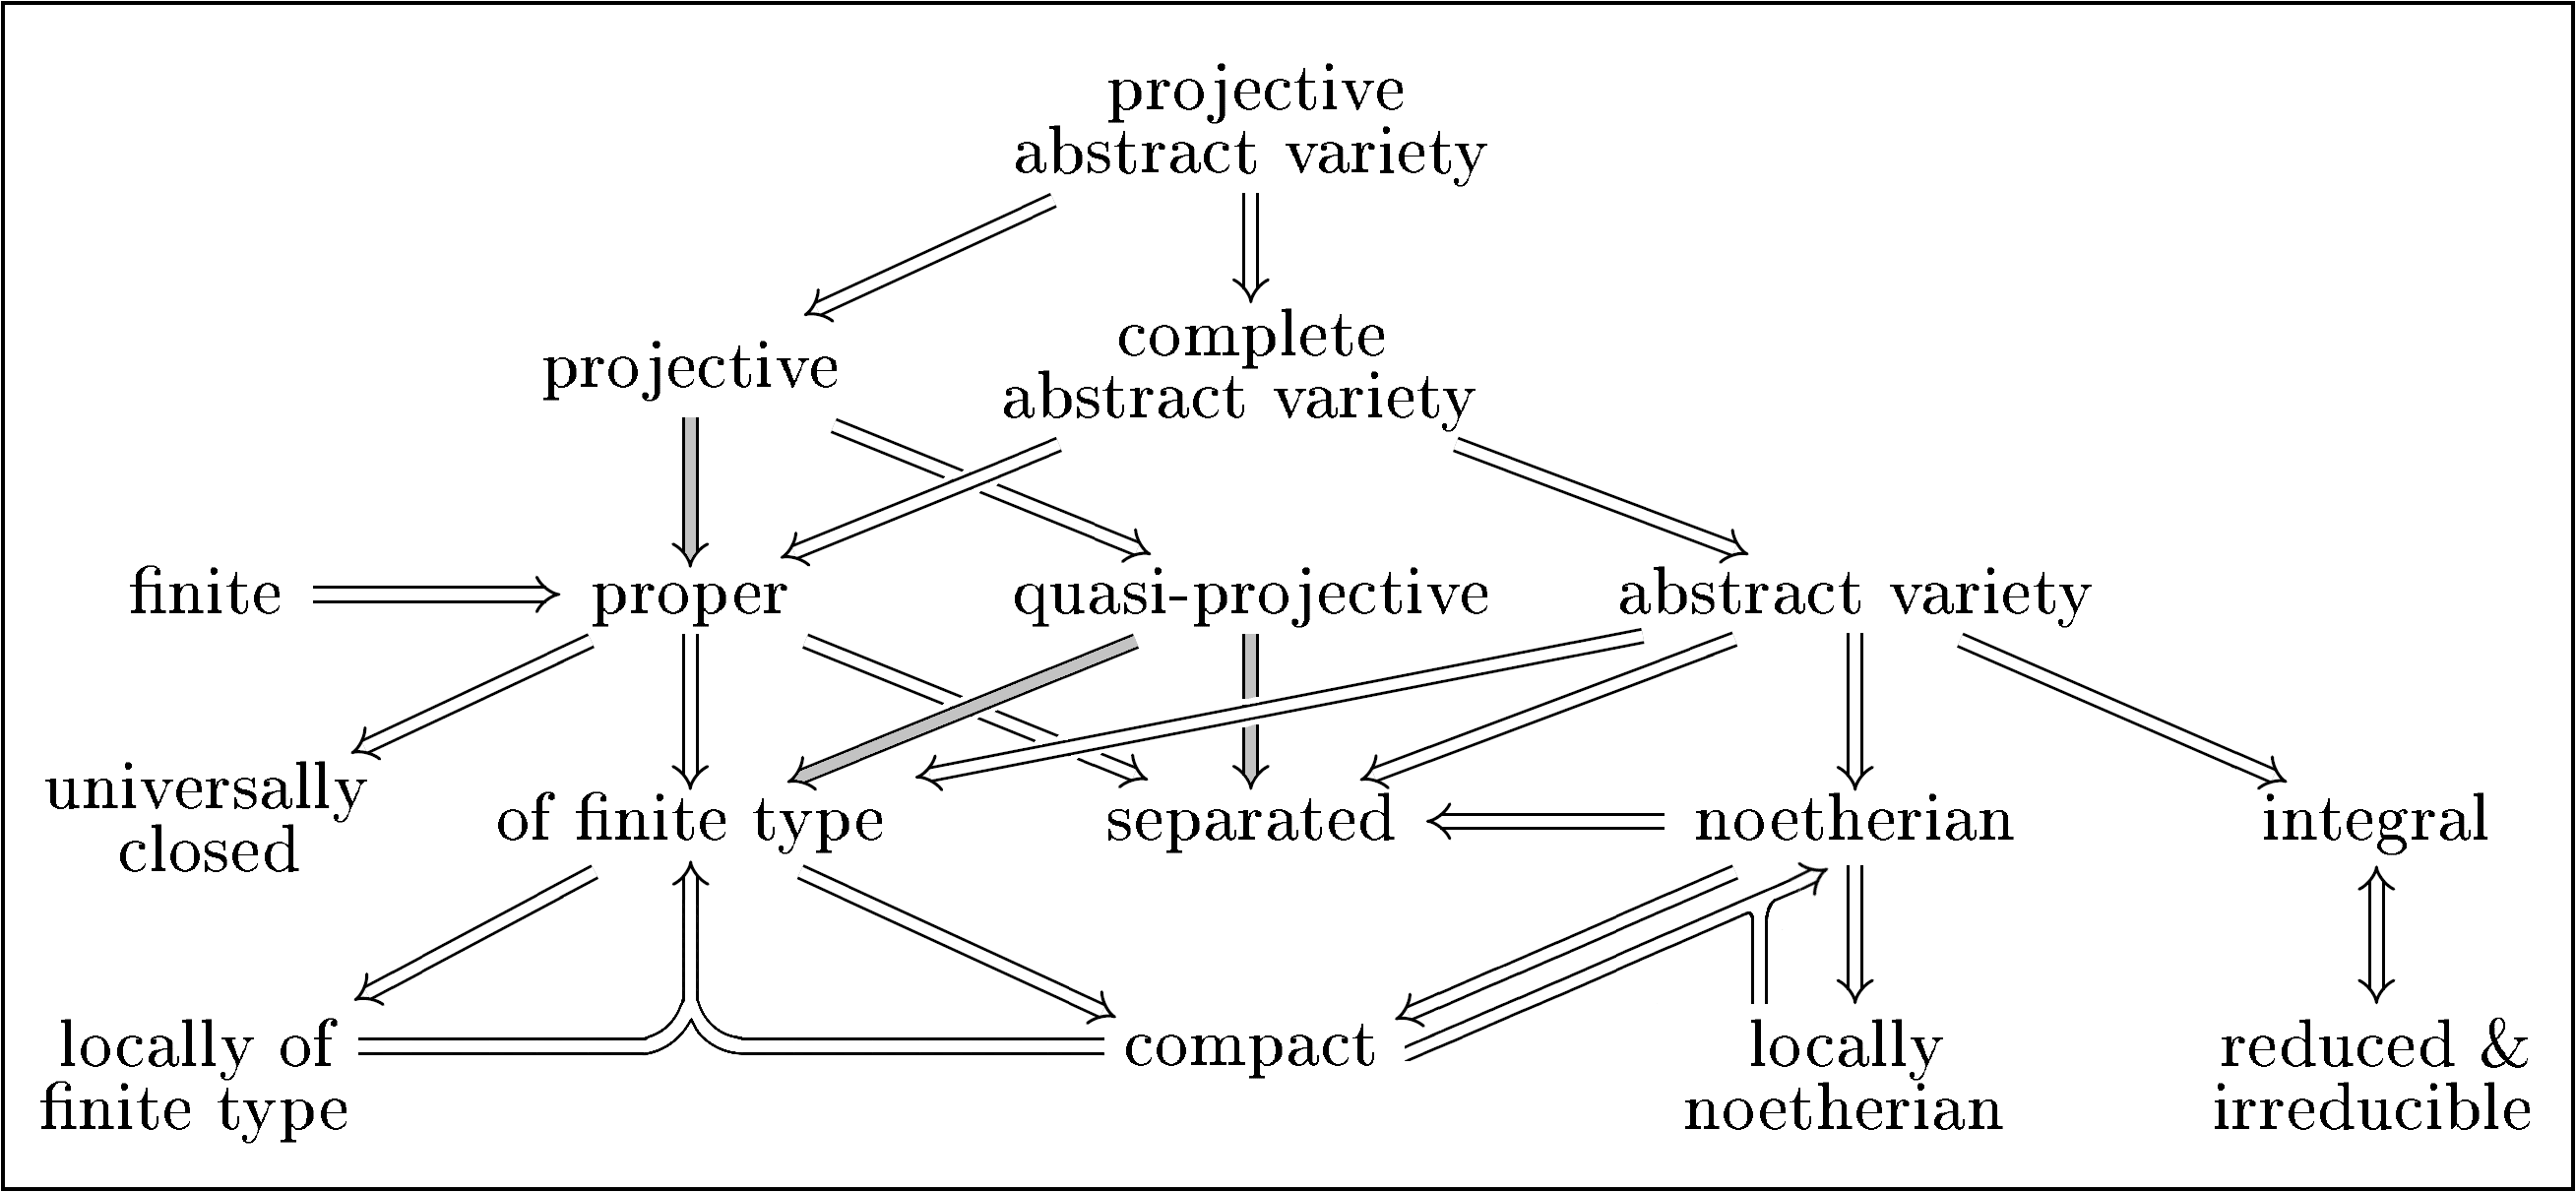
\includegraphics[width=0.95\textwidth]{bigdiagram.png}\quad
\end{figure*}\vspace*{-0.5cm}
% [Tutor Note: 原图位于原 PDF 第 79 页。紧随其后的 equation 环境（标签 bigdiagram）中保留了作者注释掉的 tikzcd 源码，故该方程本身渲染为空；此处按原样保留，便于以后直接编辑该图。]
\begin{equation}\label{bigdiagram}
%\begin{small}
%\begin{tikzpicture}[mybox/.style={draw, inner sep=1.5pt}]
%\node[mybox] (box){
%\begin{tikzcd}[column sep=1em, row sep=0.3cm]
%& & {\begin{aligned}\text{projective}\\[-0.2cm] \text{abstract variety}\end{aligned}}\arrow[dl, Rightarrow]\arrow[d, Rightarrow] & & \\
%& \text{projective}\arrow[d, Rightarrow, crossing over]\arrow[dr, Rightarrow] & {\begin{aligned}\text{complete}\\[-0.2cm] \!\!\text{abstract variety}\end{aligned}}\arrow[dr, Rightarrow]\arrow[dl, Rightarrow] &  & \\
%\text{finite}\arrow[r, Rightarrow] & \text{proper}\arrow[dl, Rightarrow]\arrow[d, crossing over, Rightarrow]\arrow[dr, crossing over, Rightarrow] & {\begin{aligned}\text{quasi-projective}\end{aligned}}\arrow[d, Rightarrow]\arrow[dl, Rightarrow] & {\begin{aligned}\text{abstract variety}\end{aligned}}\arrow[dl, Rightarrow]\arrow[d, Rightarrow]\arrow[dr, Rightarrow]  & \\
%{\begin{aligned}\text{universally}\\[-0.2cm] \!\!\text{closed}\end{aligned}} & {\begin{aligned}\text{of finite type}\end{aligned}}\arrow[dl, Rightarrow]\arrow[dr, Rightarrow]\arrow[urr, Leftarrow] & \text{separated} & \text{noetherian}\arrow[l, Rightarrow]\arrow[d, Rightarrow]\arrow[dl, Rightarrow] & \text{integral}\arrow[d, Leftrightarrow] \\
%{\begin{aligned}\text{locally of}\\[-0.2cm] \!\!\text{finite type}\end{aligned}} &  & \text{compact} & {\begin{aligned}\text{locally}\\[-0.2cm] \!\!\text{noetherian}\end{aligned}}  & {\begin{aligned}\text{reduced \&}\\[-0.2cm] \!\!\text{irreducible}\end{aligned}} 
%\end{tikzcd}
%};
%\end{tikzpicture}\end{small}
\end{equation}

最后，为后文之需，我们希望在仿射概形上的模与模层之间建立一个函子。为此，我们首先需要细化注 \ref{spectra} 中谱的结构层的构造。

\begin{Def}\label{asssheafofmodules}
设 $R$ 是环，$M$ 是（左）$R$-模，$X=\text{Spec}(R)$ 是带有结构层 $\mathcal{O}_X$ 的仿射概形。则\textbf{在 $X$ 上联系于 $M$ 的层 $\widetilde{M}$}\index{sheaf!associated to a module}由下述指定确定：
\begin{small}\begin{align*}
		\widetilde{M}(U)\!\coloneqq\!\bigg\{s\!:U\!\rightarrow\!\bigsqcup_{\mathfrak{p}\in U}\! M_\mathfrak{p}\Bigm|\, &\forall\mathfrak{p}\!\in\! U\!: s(\mathfrak{p})\!\in\! M_\mathfrak{p}\text{ and }\exists U_\mathfrak{p}\!\subset\! U\text{ $\mathfrak{p}$-neighb. }\exists m\!\in\! M\,\exists f\!\in\! R \\[-0.3cm]
		&\text{s.t. }\!\forall\mathfrak{q}\!\in\! U_\mathfrak{p}\text{ holds }f\!\notin\!\mathfrak{q} \text{ and }
		s(\mathfrak{q})\!=\! \frac{m}{f}\!\in\! M_\mathfrak{q}\bigg\}\,,
\end{align*}\end{small}
\!\!对每个开集 $U\subset X$（此处的 $M_\mathfrak{p}$ 表示 $M$ 在素理想 $\mathfrak{p}$ 处的局部化），限制映射按显然方式给出。与谱的结构层类似，可以证明确实有 $\widetilde{M}\in\text{obj}(\mathsf{Sh}(X;{}_{\mathcal{O}_X}\!\mathsf{Mod}))$。
\end{Def}

\begin{Pro}\label{squaretildefunc}
设 $R$ 是环，$M$ 是左 $R$-模，$X=\textup{Spec}(R)$ 是带有结构层 $\mathcal{O}_X$ 的仿射概形。则 $\Gamma(X,\widetilde{M})=M$，并且映射 $M\mapsto\widetilde{M}$ 确定了一个正合、全忠实的函子 $\widetilde{\square}: {}_R\mathsf{Mod}\rightarrow \mathsf{Sh}(X;{}_{\mathcal{O}_X}\!\mathsf{Mod})$。
\end{Pro}

\begin{proof}
等式 $\Gamma(X,\widetilde{M})=M$ 由对 $\Gamma(X,\mathcal{O}_X)\cong R$ 的证明稍作改编得到。其次，$\widetilde{\square}$ 是正合的，因为 $(\widetilde{M})_\mathfrak{p}\cong M_\mathfrak{p}$，而层序列的正合性可在茎的层面检验（由引理 \ref{aboutmonepisheaves}）。最后，对任意 $M, N\in\text{obj}({}_R\mathsf{Mod})$ 都有自然映射 $(\widetilde{\square})_{M,N}:\text{Hom}_R(M,N)\rightarrow\text{Hom}_{\mathcal{O}_X}(\widetilde{M},\widetilde{N})$，按我们最初的论证，其逆为 $\Gamma(X,\square)$，这就证明了它是双射，从而证明了 $\widetilde{\square}$ 的全忠实性。  
\end{proof}

事实上，还可以进一步证明 $\widetilde{\square}$ 与 $\Gamma(X,\square)$ 构成一对伴随函子：对任意 $M\in\text{obj}({}_R\mathsf{Mod})$ 与 $\mathcal{F}\in\text{obj}(\mathsf{Sh}(X;{}_{\mathcal{O}_X}\!\mathsf{Mod}))$ 有 $\text{Hom}_R(M,\Gamma(X,\mathcal{F}))\cong\text{Hom}_{\mathcal{O}_X}(\widetilde{M},\mathcal{F})$。

\begin{Rem}\label{asssheafofmodforproj}
给定分次环 $S$，可以按与定义 \ref{asssheafofmodules} 在仿射概形上的做法类似的方式，在射影谱 $X=\text{Proj}(S)$ 上对任何分次 $S$-模 $M$ 定义联系于它的层 $\widetilde{M}$。结果有 $\widetilde{M}\in\text{obj}(\mathsf{QCoh}(X;{}_{\mathcal{O}_X}\!\mathsf{Mod}))$；并且当 $S$ 诺特且 $M$ 有限生成时，还有 $\widetilde{M}\in\text{obj}(\mathsf{Coh}(X;{}_{\mathcal{O}_X}\!\mathsf{Mod}))$（由 \cite[命题 II.5.11]{[Har77]}）。

于是对任意 $n\in\mathbb{Z}$ 我们令 $\mathcal{O}_X(n)\coloneqq\widetilde{S(n)}\in\text{obj}(\mathsf{QCoh}(X;{}_{\mathcal{O}_X}\!\mathsf{Mod}))$，其中 $S(n)\coloneqq\bigoplus_{k\in\mathbb{Z}}S_{n+k}$。特别地，我们把 $\mathcal{O}_X(1)$ 称为\textit{Serre 扭层}，并把 $\mathcal{F}(n)\coloneqq\mathcal{F}\otimes_{\mathcal{O}_X}\mathcal{O}_X(n)$ 称为 $\mathcal{F}\in\text{obj}(\mathsf{Sh}(X;{}_{\mathcal{O}_X}\!\mathsf{Mod}))$ 的\textit{第 $n$ 次扭层}。

还可以通过 $\Gamma_*(\mathcal{F})\coloneqq\bigoplus_{n\in\mathbb{Z}}\Gamma(X,\mathcal{F}(n))$ 定义\textit{联系于 $\mathcal{F}$ 的分次 $S$-模}，并证明在温和的条件下它诱导出的层同构于 $\mathcal{F}$ 本身（参看 \cite[命题 II.5.15]{[Har77]}）。  
% [Tutor Note: 注意 $\mathcal{O}_X(n)$ 的记号依赖于 $\widetilde{}$ 构造对分次模的平移，即 $S(n)_{d}=S_{n+d}$；而 $\Gamma_*(\mathcal{F})$ 到 $\mathcal{F}$ 的自然映射一般不是同构，原文所谓「温和的条件」指 $S$ 由 $S_1$ 有限生成、$\mathcal{F}$ 拟凝聚等情形（详见 \cite{[Har77]} 第 II.5 节）。]
\end{Rem}

\subsection{拟凝聚层与凝聚层}\label{ch5.6}


在对概形有了更牢固的掌握之后，我们准备从第 \ref{ch5.4} 节中断之处重新拾起层论，首先给出拟凝聚层/凝聚层的另一种定义。

\begin{Rem}\label{disclaimer}(\textit{免责声明})
本节（以及余下理论的相当一部分）严重依赖概形，把由此产生的、难免更为技术性的证明推给文献，并且常常「凭信念」接受某些陈述。不过，读者可以这样自我安慰：只要知道/回想起，\cite{[Imp21]} 中 Floer 理论所提出的那些更偏分析的方面同样受到过一些重大妥协——由于时空限制与作者的无知；与此构成镜像的是，我们眼下略去的这套机制本质上是代数的——这又是镜像对称的另一种体现……总之，我们主要遵循 \cite{[Har77]}，但例如在 \cite[第 13 章]{[Vak17]} 中也能找到丰富的材料。 
\end{Rem}

\begin{Def}\label{quasi-/coherentmodules}
设 $(X,\mathcal{O}_X)$ 是概形。则 $\mathcal{F}\in\text{obj}(\mathsf{Sh}(X;{}_{\mathcal{O}_X}\!\mathsf{Mod}))$ 称为\textbf{拟凝聚 $\mathcal{O}_X$-模}\index{ox@$\mathcal{O}_X$-module!quasi-coherent}，如果 $X$ 可被一族开仿射子集 $U_i=\text{Spec}(R_i)\subset X$ 覆盖，使得对每个 $i$ 都存在 $R_i$-模 $M_i\in\text{obj}({}_{R_i}\!\mathsf{Mod})$，使 $\mathcal{F}|_{U_i}\cong\widetilde{M}_i\in\text{obj}(\mathsf{Sh}(U_i;{}_{\mathcal{O}_{U_i}}\!\mathsf{Mod}))$，其中 $\widetilde{M}_i$ 是按定义 \ref{asssheafofmodules} 联系于 $M_i$ 的层。

若每个 $M_i$ 都可选为有限生成的（从而属于 ${}_{R_i}\!\mathsf{Mod}^\mathsf{fg}\subset {}_{R_i}\!\mathsf{Mod}$），则 $\mathcal{F}$ 进一步称为\textbf{凝聚 $\mathcal{O}_X$-模}\index{ox@$\mathcal{O}_X$-module!coherent}。 

拟凝聚层/凝聚层的态射就是其底层 $\mathcal{O}_X$-模层面的态射。  
\end{Def}

我们强调，由此得到的范畴 $\mathsf{QCoh}(X;{}_{\mathcal{O}_X}\!\mathsf{Mod})$ 与 $\mathsf{Coh}(X;{}_{\mathcal{O}_X}\!\mathsf{Mod})$ 与一般环空间上的对应范畴一致——只要把定义 \ref{coherentonringed} 瞄准概形，更确切地说，在凝聚的情形瞄准诺特概形\footnote{在任意的非诺特概形上，凝聚性表现很坏。}（见 \cite[习题 II.5.4]{[Har77]}）。 

例如，任何概形 $(X,\mathcal{O}_X)$ 的结构层 $\mathcal{O}_X$ 都是凝聚 $\mathcal{O}_X$-模。
% [Tutor Note: 严格地说，「任意概形的结构层 $\mathcal{O}_X$ 都是凝聚 $\mathcal{O}_X$-模」需要（局部）凝聚性假设：在仿射情形 $X=\text{Spec}(R)$，这等价于环 $R$ 是凝聚环，并非对一切环成立。后文命题 \ref{squaretildefunctocoherent} 也只在 $R$ 诺特时给出 $\mathsf{Coh}$ 的等价，可与此对照。]

\begin{Pro}\label{squaretildefunctocoherent}
设 $R$ 是环，$X=\textup{Spec}(R)$ 是带有结构层 $\mathcal{O}_X$ 的仿射概形。则命题 \ref{squaretildefunc} 中的函子 $\widetilde{\square}:M\mapsto\widetilde{M}$ 可以改进为两个等价
\begin{equation}\label{squaretildeequivalences}
	\mkern-18mu\widetilde{\square}:{}_R\mathsf{Mod}\rightarrow\mathsf{QCoh}(X;{}_{\mathcal{O}_X}\!\mathsf{Mod})\quad\text{resp.}\quad \widetilde{\square}:{}_R\mathsf{Mod}^\mathsf{fg}\rightarrow\mathsf{Coh}(X;{}_{\mathcal{O}_X}\!\mathsf{Mod})
\end{equation}
\textup(后者在 $R$ 诺特时成立\textup)，\footnote{且不说 $\mathsf{Coh}(X;{}_{\mathcal{O}_X}\!\mathsf{Mod})$ 表现不良，当 $R$ 非诺特时我们还有 ${}_R\mathsf{Mod}^\mathsf{fg}$ \textit{不是}阿贝尔范畴——这确实相当不理想！} 二者的拟逆均为 $\Gamma(X,\square):\mathcal{F}\mapsto\Gamma(X,\mathcal{F})$。
\end{Pro}  

\begin{proof}
该陈述是下述更一般事实的推论（见 \cite[命题 II.5.4]{[Har77]}）：对一般概形 $(X,\mathcal{O}_X)$，$\mathcal{F}\in\text{obj}(\mathsf{Sh}(X;{}_{\mathcal{O}_X}\!\mathsf{Mod}))$ 是拟凝聚的，当且仅当对每个开集 $U=\text{Spec}(R_U)\subset X$ 都存在某个 $M\in\text{obj}({}_{R_U}\!\mathsf{Mod})$ 使 $\mathcal{F}|_U\cong\widetilde{M}\in\text{obj}(\mathsf{Sh}(U;{}_{\mathcal{O}_U}\!\mathsf{Mod}))$；而它在 $X$ 诺特时是凝聚的，当且仅当此外还有 $M\in\text{obj}({}_{R_U}\!\mathsf{Mod}^\mathsf{fg})$。（其实，这些只是定义 \ref{quasi-/coherentmodules} 的等价改写。）

在上式中取 $U=X$，即 $R_U=R$，就得到 $\widetilde{\square}$ 的本质满性；而 $\mathcal{O}_X$-模态射层面的全忠实性由命题 \ref{squaretildefunc} 提供（回忆：函子是等价当且仅当它全忠实且本质满）。后者同时确认 $\Gamma(X,\square)$ 是对应的拟逆。  
\end{proof}

\begin{Pro}\label{cokernelscoherent}
设 $X$ 是概形。任何拟凝聚层态射的核层、余核层与像层本身都是拟凝聚的。 

若 $X$ 还是诺特的，则任何凝聚层态射的核、余核与像也都是凝聚的。
\end{Pro}

\begin{proof}
这是局部验证，故不妨取 $X=\text{Spec}(R)$ 为仿射的。但此时 \eqref{squaretildeequivalences} 使我们能把任何拟凝聚层/凝聚层的态射视为模（分别地，有限生成模）的态射。${}_R\mathsf{Mod}$ 与 ${}_R\mathsf{Mod}^\mathsf{fg}$ 都是阿贝尔范畴（后者需 $R$ 诺特），故它们包含其任意态射的核、余核与像。再用等价 $\widetilde{\square}$ 即得命题。  
\end{proof}

作为直接推论，我们得到本节的基本结果，它使凝聚层的导出范畴之存在合法化。

\begin{Cor}\label{QCohisabelian}
对任何概形 $(X,\mathcal{O}_X)$，范畴 $\mathsf{QCoh}(X;{}_{\mathcal{O}_X}\!\mathsf{Mod})$ 都是阿贝尔范畴；而对任何诺特概形 $(X,\mathcal{O}_X)$，范畴 $\mathsf{Coh}(X;{}_{\mathcal{O}_X}\!\mathsf{Mod})$ 都是阿贝尔范畴。
\end{Cor}

\begin{proof}
由于 $\mathsf{QCoh}(X;{}_{\mathcal{O}_X}\!\mathsf{Mod})$ 与 $\mathsf{Coh}(X;{}_{\mathcal{O}_X}\!\mathsf{Mod})$ 都是阿贝尔范畴 $\mathsf{Sh}(X;{}_{\mathcal{O}_X}\!\mathsf{Mod})$ 的全子范畴，只需验证它们对有限直和与余核/核封闭。后者由命题 \ref{cokernelscoherent} 提供；至于前者，我们注意到：给定两个拟凝聚层/凝聚层 $\mathcal{F}, \mathcal{G}$ 以及它们共同的开覆盖 $\{U_i\}_{i\in I}$，局部地有 $(\mathcal{F}\oplus\mathcal{G})|_{U_i}=\mathcal{F}|_{U_i}\oplus\mathcal{G}|_{U_i}\cong \widetilde{M}_i\oplus\widetilde{N}_i\cong(\widetilde{M\oplus N})_i$（对合适的模），从而 $\mathcal{F}\oplus\mathcal{G}$ 也是拟凝聚的/凝聚的。最后，零层显然是拟凝聚的/凝聚的。
% [Tutor Note: 这里用到的判据是：阿贝尔范畴的全子范畴若对有限直和（从而含零对象）以及核、余核封闭，则它自身是阿贝尔范畴，且包含函子是正合的。末句「零层显然拟凝聚」正是补上零对象这一条。]
\end{proof}

\begin{Rem}\label{desirablecoherentprop}
让我们强调哪些良好的性质在拟凝聚性/凝聚性下得以保持。设 $(X,\mathcal{O}_X)$ 是概形。
\begin{itemize}[leftmargin=0.5cm]
	\item 给定拟凝聚层 $\mathcal{F}$，Hom 群与局部 $\mathcal{H}om$-层给出
	\begin{equation}\label{locHomonqcoh}
		\begin{aligned}
			&\text{Hom}_{\mathcal{O}_X}\!(\mathcal{F},\square):\mathsf{QCoh}(X;{}_{\mathcal{O}_X}\!\mathsf{Mod})\rightarrow \mathsf{Ab}\,, \\
			&\mathcal{H}om_{\mathcal{O}_X}\!(\mathcal{F},\square):\mathsf{QCoh}(X;{}_{\mathcal{O}_X}\!\mathsf{Mod})\rightarrow \mathsf{QCoh}(X;{}_{\mathcal{O}_X}\!\mathsf{Mod})\,, 
		\end{aligned}
	\end{equation}
	二者都是左正合的。若 $\mathcal{F}$ 还是凝聚层，则这些函子特化为左正合的
	\begin{equation}\label{locHomoncoh}
		\begin{aligned}
			&\text{Hom}_{\mathcal{O}_X}\!(\mathcal{F},\square):\mathsf{Coh}(X;{}_{\mathcal{O}_X}\!\mathsf{Mod})\rightarrow \mathsf{Vect}_\mathbb{K}\,, \\
			&\mathcal{H}om_{\mathcal{O}_X}\!(\mathcal{F},\square):\mathsf{Coh}(X;{}_{\mathcal{O}_X}\!\mathsf{Mod})\rightarrow \mathsf{Coh}(X;{}_{\mathcal{O}_X}\!\mathsf{Mod})
		\end{aligned}
	\end{equation}
	（其中对 Hom 我们还进一步假定了 $X\in\text{obj}(\mathsf{Sch}(\mathbb{K}))$ 是射影的，并用 $\mathsf{Vect}_\mathbb{K}$ 记 $\mathbb{K}$ 上有限维向量空间的范畴）。
	\newline 类似地，我们有反变左正合函子 $\text{Hom}_{\mathcal{O}_X}\!(\square,\mathcal{F})$ 与 $\mathcal{H}om_{\mathcal{O}_X}\!(\square,\mathcal{F})$。特别地，凝聚层 $\mathcal{F}$ 的对偶层 $\mathcal{F}^\vee=\mathcal{H}om_{\mathcal{O}_X}\!(\mathcal{F},\mathcal{O}_X)$ 也是凝聚的。
	
	\item 张量运算对拟凝聚层/凝聚层同样表现良好，给出右正合函子 \begin{equation}\label{tensoronqcoh}
		\begin{aligned}
			&\mathcal{F}\otimes_{\mathcal{O}_X}\!\square:\mathsf{QCoh}(X;{}_{\mathcal{O}_X}\!\mathsf{Mod})\rightarrow \mathsf{QCoh}(X;{}_{\mathcal{O}_X}\!\mathsf{Mod})\,, \\
			&\square\!\otimes_{\mathcal{O}_X}\mathcal{G}:\mathsf{QCoh}(X;\mathsf{Mod}_{\mathcal{O}_X})\rightarrow \mathsf{QCoh}(X;{}_{\mathcal{O}_X}\!\mathsf{Mod})\,,
		\end{aligned}
	\end{equation}
	其中分别要求 $\mathcal{F}\in\text{obj}(\mathsf{QCoh}(X;\mathsf{Mod}_{\mathcal{O}_X}))$ 与 $\mathcal{G}\in\text{obj}(\mathsf{QCoh}(X;{}_{\mathcal{O}_X}\!\mathsf{Mod}))$；当 $\mathcal{F},\mathcal{G}$ 分别是凝聚的右、左 $\mathcal{O}_X$-模时，则给出右正合的
	\begin{equation}\label{tensoroncoh}
		\begin{aligned}
			&\mathcal{F}\otimes_{\mathcal{O}_X}\!\square:\mathsf{Coh}(X;{}_{\mathcal{O}_X}\!\mathsf{Mod})\rightarrow \mathsf{Coh}(X;{}_{\mathcal{O}_X}\!\mathsf{Mod})\,, \\
			&\square\!\otimes_{\mathcal{O}_X}\mathcal{G}:\mathsf{Coh}(X;\mathsf{Mod}_{\mathcal{O}_X})\rightarrow \mathsf{Coh}(X;{}_{\mathcal{O}_X}\!\mathsf{Mod})\,,
		\end{aligned}
	\end{equation}。
	\newline 注意在仿射的 $X=\text{Spec}(R)$ 上有 $\Gamma(X,\mathcal{F}\otimes_{\mathcal{O}_X}\!\mathcal{G})\cong\Gamma(X,\mathcal{F})\otimes_R \Gamma(X,\mathcal{G})$。这可用来定义并证明拟凝聚层的张量幂、对称幂与外幂都是拟凝聚的。
	
	\item 给定拟凝聚层的短正合序列 $0\rightarrow\mathcal{F}_1\rightarrow\mathcal{F}_2\rightarrow\mathcal{F}_3\rightarrow 0$，若 $\mathcal{F}_1$ 与 $\mathcal{F}_3$ 也是局部自由的，则 $\mathcal{F}_2$ 也必局部自由（在仿射子集上，对自由层有同样的结论）。
	\newline 再假设 $X$ 是诺特的，并设 $\mathcal{F}$ 是凝聚 $\mathcal{O}_X$-模。则 $\mathcal{F}$ 局部自由当且仅当对每个 $x\in X$，$\mathcal{F}_x$ 是自由 $\mathcal{O}_{X,x}$-模；而它是可逆层当且仅当存在另一个凝聚层 $\mathcal{G}$ 使 $\mathcal{F}\otimes_{\mathcal{O}_X}\!\mathcal{G}\cong\mathcal{O}_X$。 
\end{itemize}
% [Tutor Note: 上一条中原文混用了 $\mathsf{QCoh}(X;\mathsf{Mod}_{\mathcal{O}_X})$ 与 $\mathsf{QCoh}(X;{}_{\mathcal{O}_X}\!\mathsf{Mod})$ 两种写法，二者指同一个范畴（左 $\mathcal{O}_X$-模层）；张量积两端的模结构（右、左）也须与之匹配，此处照原文保留。]
\end{Rem}

特别有用的是弄清拉回与推前函子如何与拟凝聚层/凝聚层相互作用。回顾上一节的众多定义，我们有：

\begin{Pro}\label{pushpullcoherent}
设 $f:(X,\mathcal{O}_X)\rightarrow (Y,\mathcal{O}_Y)$ 是概形态射 \textup(从而是底层局部环空间的态射；参看定义 \ref{locallyringedspace}\textup)。则：
\renewcommand{\theenumi}{\roman{enumi}}
\begin{enumerate}[leftmargin=0.6cm]
	\item 拉回函子特化为 $f^*\!\!: \mathsf{QCoh}(Y;{}_{\mathcal{O}_Y}\!\mathsf{Mod})\!\rightarrow\!\mathsf{QCoh}(X;{}_{\mathcal{O}_X}\!\mathsf{Mod})$，并且当 $X$、$Y$ 都诺特时，特化为 $f^*\!: \mathsf{Coh}(Y;{}_{\mathcal{O}_Y}\!\mathsf{Mod})\rightarrow \mathsf{Coh}(X;{}_{\mathcal{O}_X}\!\mathsf{Mod})$。二者都是右正合的。
	
	\item 若 $X$ 诺特，或 $f$ 分离且紧，则推前函子特化为左正合的 $f_*\!: \mathsf{QCoh}(X;{}_{\mathcal{O}_X}\!\mathsf{Mod})\!\rightarrow \!\mathsf{QCoh}(Y;{}_{\mathcal{O}_Y}\!\mathsf{Mod})$。 
	\newline 此外，若 $f$ 是诺特概形之间的有限态射，或是域 $\mathbb{K}$ 上有限型概形之间的射影态射——更一般地，若 $f$ 是诺特概形之间的固有态射——则它诱导左正合的 $f_*: \mathsf{Coh}(X;{}_{\mathcal{O}_X}\!\mathsf{Mod})\rightarrow \mathsf{Coh}(Y;{}_{\mathcal{O}_Y}\!\mathsf{Mod})$。  
\end{enumerate}
\end{Pro}

\begin{proof}(\textit{概要})
关于拉回，问题是局部的，故可设 $X$ 与 $Y$ 都是仿射的。于是应用命题 \ref{squaretildefunctocoherent} 以及 \cite[命题 II.5.2]{[Har77]} 即得第 \textit{i} 点。注意 $f^*=\mathcal{O}_X\otimes_{f^{\!-\!1}\!\mathcal{O}_Y}\! f^{-1}(\square)$ 的右正合性继承自 $f^{-1}$ 与张量积的右正合性。 

关于推前，按假设可取 $Y$ 为仿射的，并用有限多个开仿射子集覆盖 $X$（因为 $f$ 是紧的）。于是为证明对任意 $\mathcal{F}\in\text{obj}(\mathsf{QCoh}(X;{}_{\mathcal{O}_X}\!\mathsf{Mod}))$ 有 $f_*\mathcal{F}\in\text{obj}(\mathsf{QCoh}(Y;{}_{\mathcal{O}_Y}\!\mathsf{Mod}))$，只需利用：任意一对拟凝聚层 $\mathcal{G}_1,\mathcal{G}_3$ 的扩充 $\mathcal{G}_2$——按定义，它装入短正合序列 $0\rightarrow\mathcal{G}_1\rightarrow\mathcal{G}_2\rightarrow\mathcal{G}_3\rightarrow 0$——本身也是拟凝聚的（见 \cite[命题 II.5.7]{[Har77]}）。 

把 $f_*$ 限制到凝聚层上，我们只说明 $f$ 为射影的情形如何证明：由局部性，取 $Y=\text{Spec}(A)$，其中 $A$ 是有限生成的 $\mathbb{K}$-代数（从而是环），于是对任意 $\mathcal{F}\in\text{obj}(\mathsf{Coh}(X;{}_{\mathcal{O}_X}\!\mathsf{Mod}))$，前一点已保证 $f_*\mathcal{F}$ 是拟凝聚的；再由命题 \ref{squaretildefunctocoherent} 有 $f_*\mathcal{F}\cong(\widetilde{\square}\circ\Gamma(Y,\square))(f_*\mathcal{F})=\widetilde{\square}\big(\mathcal{F}(f^{-1}(Y))\big)=\Gamma(X,\mathcal{F})^\sim$，而它实际上是凝聚的，因为 $\Gamma(X,\mathcal{F})$ 是有限生成的 $A$-模（由 \cite[定理 II.5.19]{[Har77]}）。$f$ 固有时的更一般证明见 \cite[第 III.8 节]{[Har77]}。  
\end{proof}
% [Tutor Note: 值得强调 $f_*$ 一般\emph{并不}保持拟凝聚性：原文给出的两个充分条件（$X$ 诺特，或 $f$ 分离且紧）都不可省；完整证明被推给 \cite{[Har77]} 第 II.5 节与第 III.8 节。另外 $f^*$ 的右正合性与 $f_*$ 的左正合性，也可由它们构成伴随对（同构 \eqref{pullpushareadjoints}）直接读出。]

注意 $f^*$ 与 $f_*$ 的右、左正合性同样可由它们构成一对伴随函子推出（见同构 \eqref{pullpushareadjoints}），即使在拟凝聚/凝聚的世界里也是如此。

\begin{Cor}\label{globalsectforcoherent}
设 $X$ 是诺特概形。则引理 \ref{sectfuncexact} 的整体截面函子 \textup(取 $U=X$ 时\textup)特化为左正合函子：
\begin{equation}
	\begin{aligned}
		&\Gamma(X,\square): \mathsf{QCoh}(X;{}_{\mathcal{O}_X}\!\mathsf{Mod})\rightarrow\mathsf{Ab}\,, \\
		&\Gamma(X,\square):\mathsf{Coh}(X;{}_{\mathcal{O}_X}\!\mathsf{Mod})\rightarrow\mathsf{Ab}\,.
	\end{aligned}
\end{equation}
特别地，若 $X\in\textup{obj}(\mathsf{Sch}(\mathbb{K}))$ 是 $\mathbb{K}$ 上的诺特概形，分别地是射影的\textup(或仅为固有的\textup)概形，则我们有左正合函子：
\begin{equation}\label{globsectsfunconcoh}
	\begin{aligned}
		&\Gamma(X,\square):\mathsf{QCoh}(X;{}_{\mathcal{O}_X}\!\mathsf{Mod})\rightarrow\mathsf{Vect}_\mathbb{K}^{\leq\infty}\,, \\
		&\Gamma(X,\square):\mathsf{Coh}(X;{}_{\mathcal{O}_X}\!\mathsf{Mod})\rightarrow\mathsf{Vect}_\mathbb{K}
	\end{aligned}
\end{equation}
\textup(其中 $\mathsf{Vect}_\mathbb{K}^{\leq\infty}$ 是可能无穷维的 $\mathbb{K}$-向量空间所成的范畴\textup)。 
\end{Cor}

\begin{proof}
这由命题 \ref{pushpullcoherent} 直接得到：只需取\footnote{在下文注 \ref{sectfuncispushforward} 中我们将看到，对模层也有同样的结论，只要把目标空间取为配以合适常层的单点空间。} $Y=\text{Spec}(\mathbb{K})$，并取 $f:X\rightarrow \text{Spec}(\mathbb{K})$ 为结构态射，它在 $\mathbb{K}$ 上是固有的。再由引理 \ref{sectfuncexact} 即得左正合性。 

若 $X$ 在 $\mathbb{K}$ 上射影，则上一个证明已经提示：对任意 $\mathcal{F}\in\text{obj}(\mathsf{Coh}(X;{}_{\mathcal{O}_X}\!\mathsf{Mod}))$，$\Gamma(X,\mathcal{F})$ 是有限生成的 $\mathbb{K}$-模（这一事实在定理 \ref{sheafcohomforprojsch} 的证明中有更一般的说明），即有限维 $\mathbb{K}$-向量空间。放松到拟凝聚层，我们只是允许无限维的向量空间出现。
\end{proof}


\newpage
\pagestyle{fancy}

